% Created 2014-11-28 Fri 11:53
\documentclass[t,xcolor=dvipsnames,english,bigger,aspectratio=43,hyperref={unicode=true}]{beamer}

% Required packages
\usepackage{tikz}
\usepackage{ifthen}
\usepackage[T1]{fontenc}
\usetikzlibrary{arrows,positioning,intersections,shadows,shapes}
\usepackage{tikz}
\usepackage{color}
\usepackage{tcolorbox}
\usepackage{caption}
\usepackage{subcaption}
\usepackage[export]{adjustbox}
\usepackage{graphicx}
\usepackage{fancybox}
\usepackage{varwidth}
\usepackage{pgfplots}
\pgfplotsset{compat = newest}
%\usepgfplotslibrary{colorbrewer}
%\pgfplotstableread{ave_rate_new.txt}
%\datatable
\definecolor{skyblue1}{rgb}{0.447,0.624,0.812}
\definecolor{scarletred1}{rgb}{0.937,0.161,0.161}

\definecolor{s1}{RGB}{228, 26, 28}
\definecolor{s2}{RGB}{55, 126, 184}
\definecolor{s3}{RGB}{77, 175, 74}
\definecolor{s4}{RGB}{152, 78, 163}
\definecolor{s5}{RGB}{255, 127, 0}

 \tikzset{
    invisible/.style={opacity=0},
    visible on/.style={alt={#1{}{invisible}}},
    alt/.code args={<#1>#2#3}{%
      \alt<#1>{\pgfkeysalso{#2}}{\pgfkeysalso{#3}} % \pgfkeysalso doesn't change the path
    },
  }

\usetikzlibrary{shapes,snakes}
\usepackage{amsmath,amssymb}

\usetikzlibrary{positioning}
\usepackage{rotating}
\usetikzlibrary{chains}
\usepackage{epstopdf}

\pgfmathsetmacro{\myinnersep}{2}% inner sep in mm

\tikzset{
box/.style={draw,%
        inner sep=\myinnersep,%
        outer sep=0,%
    minimum width=5mm,%
    minimum height=\heightof{Cap}+1.8*\myinnersep*1mm,%
    align=center}
}

\usetikzlibrary{decorations.pathmorphing} % for snake lines
\usetikzlibrary{matrix} % for block alignment
\usetikzlibrary{arrows} % for arrow heads
\usetikzlibrary{calc} % for manimulation of coordinates
\usepackage{multirow}

% Font definitions; uncomment if you want to change fonts. You'll need the
% specified fonts installed. Compile with xelatex or lualatex for this to work.
% The Helvetica Neue and Calibri fonts are in the fonts/ directory, but need to
% be installed on the system (Linux: drop them in ~/.fonts - Mac & Windows:
% install through the system font management utility).
\usepackage{fontspec}
\usepackage{unicode-math}
\defaultfontfeatures{Ligatures=TeX}
\setmainfont[
  BoldFont={HelveticaNeueLTStd-Bd},
  BoldItalicFont={HelveticaNeueLTStd-BdIt},
  ItalicFont={HelveticaNeueLTStd-It}]{Helvetica Neue LT Std}
\setmonofont[Scale=0.8]{Inconsolata}
\setsansfont{Calibri}

% For non-Xe/Lua-latex compilation
%\usepackage[utf8]{inputenc}



% Beamer settings
% The files beamer*themecsdv.sty and
% kau_2012_cmyk_eps_14679.pdf need to be in the same directory as the .tex file,
% or in $TEXINPUTS, for the template to work.

%\beamerdefaultoverlayspecification{<+->}
\usetheme{csdv}

% Author information
\author{M. Rajiullah}
\authoremail{mohammad.rajiullah@kau.se}
\date{\today}
\title{\LARGE{HTTP over TCP or SCTP}\\ KaU, UoA, FHM, Mozilla}



\begin{document}

\maketitle
%\begin{frame}{Outline}
%\tableofcontents
%\end{frame}

%%====================%%
\begin{frame}{Goal}
%\begin{itemize}
%\item Investigate the usefulness of alternative transports for web traffic, and to understand how transport mechanisms impact performance of web %traffic.
%\end{itemize}
 \vfill
\begin{center}
\begin{tcolorbox}[colback=green!5,colframe=green!40!black]
Investigate the usefulness of alternative transports for web traffic, and to understand 
how/what specific transport mechanisms impact the most.
\end{tcolorbox}
\end{center}
 \vfill
\end{frame}
%%====================%%
\begin{frame}{Web traffic over alternative transports}
\begin{itemize}
\item Hypothesis: Multistreaming in single SCTP connection can improve the web browsing perfromance 
as compared to multiple TCP connections used in today's browser
\item Existing work~\cite{Natarajan06,Natarajan08,Natarajan09,Xue09} has already evaluated SCTP web performance
\item We will extend their basic analysis by evaluating over a wider range of network scenarios and modern 
and realistic workload.
\end{itemize}
\end{frame}
%%====================%%
\begin{frame}{Development of experimental tools}
\begin{itemize}
\item \textit{pReplay}: A tool that can replay web page loading (Kau+FHM) \\
\color{red} ./pReplay server testfile [http|https|http2|phttpget] [max-connections] [cookie-size] \color{black}
\item thttpd (patch)  SCTP multistreaming, TCP Persistency/Keep-Alive support, 
Keep-Alive support on HTTP response 404,403 (UoA+FHM) 
\end{itemize}
\end{frame}
%%====================%%
\begin{frame}{Experiment Setup}
\tiny
\begin{table}[t!]
\label{tab:exp_param}
  \centering
\begin{tabular}{|l|l|l|}

\hline
\multicolumn{3}{|c|}{Experiment parameters} \\
\hline
Category & Factor & Range/value \\ \hline
\multirow{3}{*}{Network} & RTTs & Desktop users (20, 79, 194, 800 ms), mobile users (44, 94, 184, 913 ms)\\
 &&in 25, 50, 75 and 95th percentile  \\
 & Banwidth & Unlimited, DSL 10Mbps, 3G 1Mbps\\
 & Packet loss & No loss, 1.5\%, 3\% \\ \hline
\multirow{3}{*}{TCP/SCTP} & IW & client (iw 3), server (iw 10) \\
 & CWND validation & no \\
 & Parallel TCPs & 1, 6, 18 \\ \hline
\multirow{2}{*}{Webpage} & Sets & small, medium, large  \\
 & Cookie in the request & NULL, 512 B, 2K \\
\hline
\end{tabular}
\caption{Experiment parameters}
\end{table}


\centering
\begin{tikzpicture}[scale=0.7,
    start chain=going right,
    diagram item/.style={
        on chain,
        join
    }
]
\node [
    diagram item,
    label=below:Client (Linux)
] {
\includegraphics{imgs/pc}};

\node [
    diagram item,
    label=below:Dummynet (FreeBSD)
] {
\includegraphics{imgs/pc}};

\node [
    diagram item,
    label=below:Server (FreeBSD)
] {
\includegraphics{imgs/pc}};
\end{tikzpicture}

\end{frame}
%%====================%%
\begin{frame}{Results}
\begin{columns}[t]
\column{.5\textwidth}
\centering
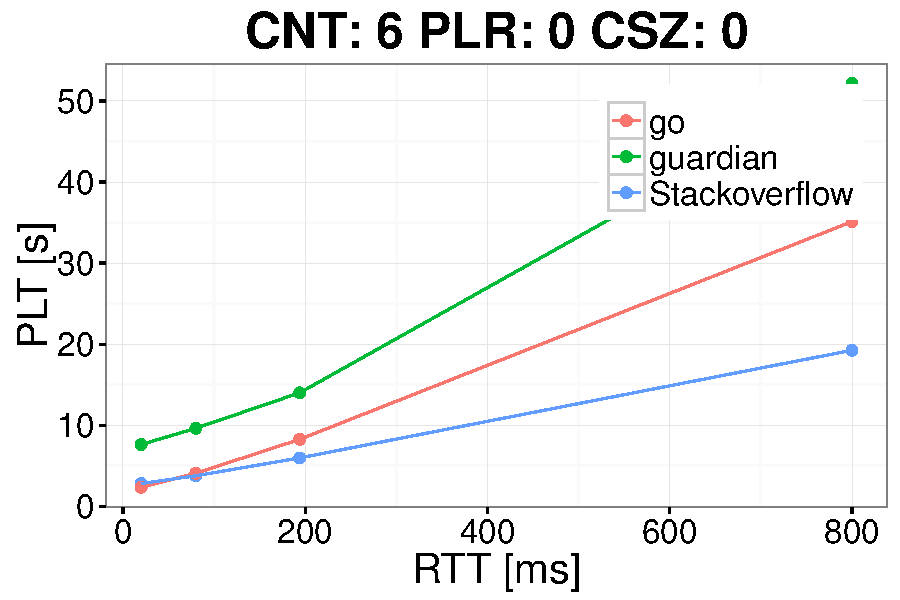
\includegraphics[width=5cm,height=3.5cm]{imgs/rtt}\\
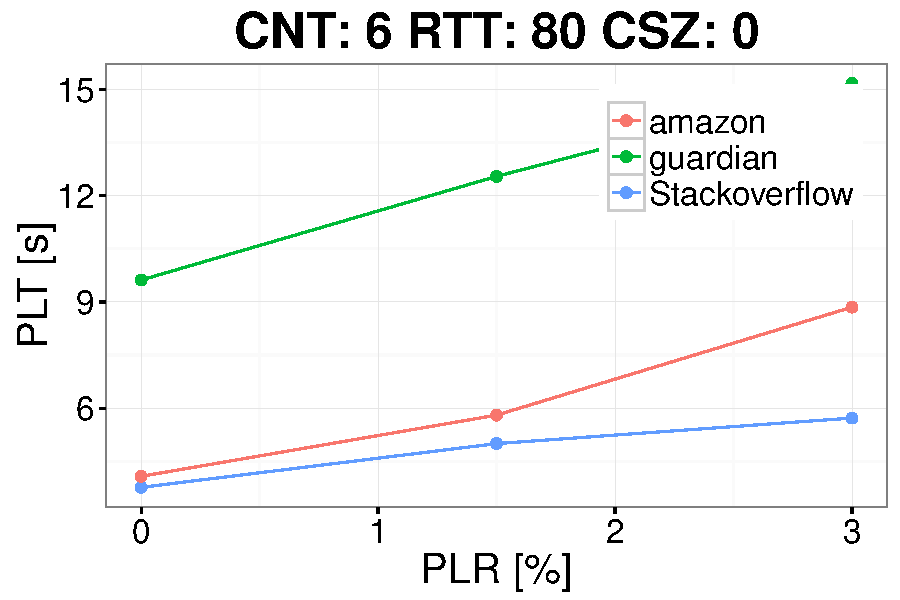
\includegraphics[width=5cm,height=3.5cm]{imgs/plr}
\column{.5\textwidth}
\centering
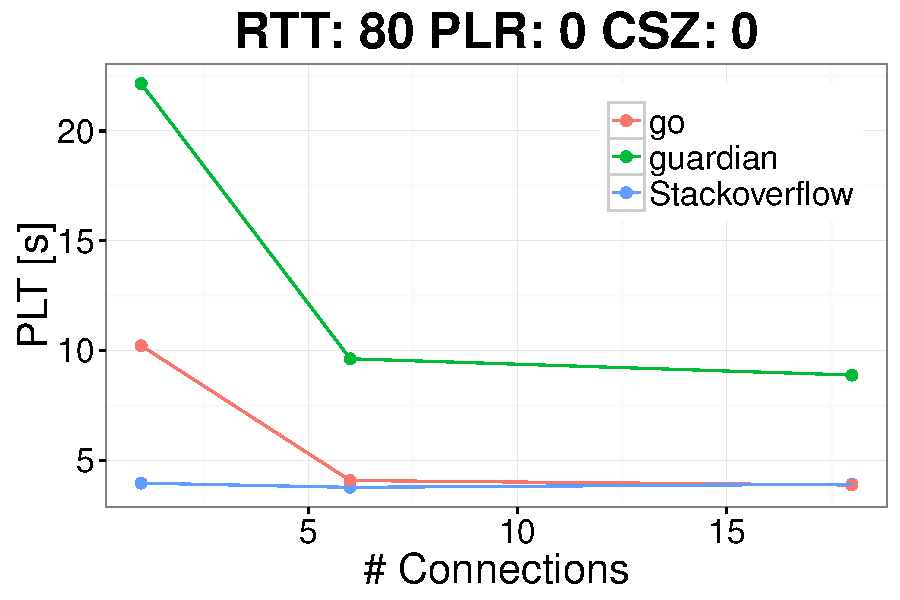
\includegraphics[width=5cm,height=3.5cm]{imgs/cnt}\\
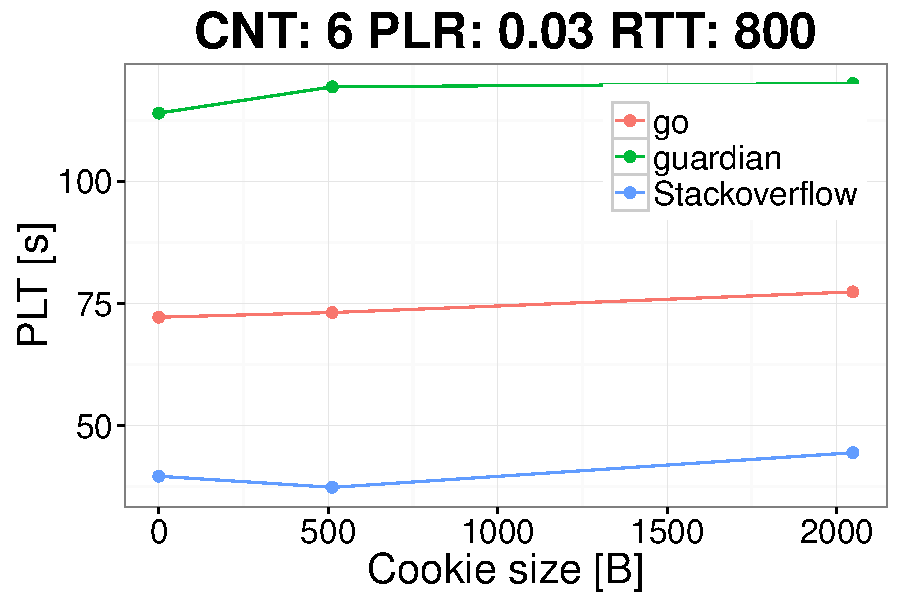
\includegraphics[width=5cm,height=3.5cm]{imgs/csz}
\end{columns}

\end{frame}
%%====================%%
\begin{frame}{Results contd.}
\begin{itemize}
\item For all combinations, if RTT increases web loading time increases
\item Similarly, if loss increases, web loading time increases
\item Increasing the number of parallel TCPs from 1 to 6 reduces web load time in all cases, 
but increasing it any further only favours large site, guardian occasionally
\item  Influence from different cookie sizes are not clearly visible
\end{itemize}
\end{frame}
%%====================%%
\begin{frame}{Next steps}
\begin{itemize}
\item Debug phttpget 
\item Compare the results with TCP against SCTP (multistreaming)
\item Possible outcome: publishing a paper with the results from the experiments
\end{itemize}
\end{frame}
%%====================%%
\begin{frame}{References}
\tiny
  %\scriptsize
\bibliographystyle{ieeetr}
\bibliography{h1_over_tcp_or_sctp}
\end{frame}

\end{document}
